\documentclass[conference]{IEEEtran}
\usepackage{cite}
\usepackage{amsmath,amssymb,amsfonts}
\usepackage{graphicx}
\usepackage{booktabs}
\usepackage{url}

% ============================================================
% REVISED MANUSCRIPT — restructured per review pass 2026-07-13
% Original main.tex untouched. All numerical values identical
% to the original. TODOs marked below must be resolved before
% submission (search for "TODO").
% ============================================================

\begin{document}

\title{When Enhancement Becomes an Attack:\\
DWT-DCT Watermark Robustness Under AI Super-Resolution}

\author{\IEEEauthorblockN{Shiva Tan}
\IEEEauthorblockA{Independent Researcher\\
your.email@example.com}} % TODO: real email

\maketitle

\begin{abstract}
Classical DWT-DCT image watermarking remains widely deployed in
forensic and broadcast systems. Its robustness evaluation has
historically rested on an implicit assumption: destroying an embedded
watermark requires visibly degrading the image. We investigate whether
AI-based image enhancement violates this assumption. Across 100 images
from the Kodak and TAMPERE17 datasets at four embedding strengths,
Real-ESRGAN super-resolution reduces mean normalized correlation (NC)
from 0.999 to 0.795 (bit error rate 0.103) while producing the highest
perceptual quality of any attack tested (SSIM 0.906) --- a
high-quality, low-detection region that no classical attack reaches.
ESPCN, which shares the identical $4\times$ upscale and Lanczos
downscale pipeline, leaves watermarks nearly intact (NC 0.999),
indicating the effect arises from the learned reconstruction itself
rather than from resampling or from AI enhancement in general. A
coefficient-stability analysis across 102,400 DCT blocks shows that
Real-ESRGAN concentrates perturbation in the DC coefficient at 5 to 14
times the magnitude of any other position, whereas JPEG distributes
damage nearly uniformly --- mechanistically distinct profiles that
help explain why compression-oriented benchmarks do not predict
enhancement vulnerability. Guided by this profile, a structured sweep
of 43 coefficient pairs shows that repositioning embedding to
$(7,5)/(7,7)$ improves Real-ESRGAN robustness (NC 0.795 to 0.833) and
raises minimum PSNR above the 40\,dB imperceptibility threshold, at
the cost of JPEG robustness (0.996 to 0.903); no configuration
improves against all attacks simultaneously. Our results suggest that
AI enhancement should be treated as a first-class attack category in
watermarking robustness evaluation, and that attack-aware coefficient
selection offers partial but not complete mitigation.
\end{abstract}

\begin{IEEEkeywords}
digital watermarking, DWT-DCT, image forensics, robustness evaluation,
super-resolution, AI enhancement, Real-ESRGAN
\end{IEEEkeywords}

\section{Introduction}
\label{sec:intro}

Robustness evaluation for classical image watermarking rests on a
quality--attack tradeoff: the standard benchmark attacks --- JPEG
compression, additive noise, filtering, geometric distortion
\cite{petitcolas1998,cox2007} --- all degrade image quality in
proportion to the damage they inflict on the watermark. An attacker
who wishes to remove a watermark must accept perceptible image damage.
This assumption is not incidental; it directly informs how embedding
positions and strengths are chosen in deployed systems, and it defines
what ``robust'' has meant in three decades of evaluation practice.

This paper asks a single question: \emph{does consumer AI-based image
enhancement violate this assumption for classical DWT-DCT
watermarking --- and if so, why, and what can be done about it within
the classical scheme?}

The question is practically urgent. Combined DWT-DCT watermarking
\cite{alhaj2007} remains a canonical choice in cameras, broadcast
equipment, and digital asset management, valued for computational
simplicity and independence from machine-learning infrastructure, and
it continues to serve as the classical baseline in watermarking
research \cite{waves2024}. Meanwhile, super-resolution models such as
Real-ESRGAN \cite{realesrgan2021} are embedded in consumer photo
tools. A user who ``enhances'' a watermarked photograph may degrade
the embedded signal with no forensic intent and --- critically --- no
visible indication that anything was altered. Whether this constitutes
a meaningful threat to deployed classical schemes has not been
systematically studied: the WAVES benchmark \cite{waves2024} evaluated
DWT-DCT only in an appendix and included no enhancement-class attacks,
and W-Bench \cite{wbench2024} evaluates only neural watermarks.

We answer the question in three stages, which structure the paper.
\emph{Observation} (Section~\ref{sec:results}): Real-ESRGAN reduces
mean NC to 0.795 while achieving SSIM of 0.906, the highest perceptual
quality of any attack we test --- a combination absent from every
classical attack profile. ESPCN \cite{espcn2016}, passed through the
identical upscale--downscale pipeline, leaves watermarks intact,
isolating the cause to the learned reconstruction.
\emph{Mechanism} (Section~\ref{sec:analysis}): a stability analysis
over 102,400 DCT blocks shows Real-ESRGAN concentrates damage in the
DC coefficient at 5--14$\times$ the magnitude of any other position,
whereas JPEG spreads damage uniformly --- a perturbation profile under
which the classical embedding positions, chosen for compression-era
attacks, are no longer well placed.
\emph{Design implication and validation}
(Section~\ref{sec:analysis}): if the damage profile is
attack-specific, coefficient selection should be attack-aware. A sweep
of 43 coefficient pairs confirms partial mitigation is achievable ---
positions $(7,5)/(7,7)$ improve Real-ESRGAN NC from 0.795 to 0.833 and
eliminate imperceptibility failures --- but at a quantified cost to
JPEG robustness, with no configuration improving against all attacks
simultaneously.

Our contributions are:
\begin{itemize}
\item To the best of our knowledge, the first systematic evaluation of
a classical DWT-DCT scheme under learned super-resolution,
demonstrating that AI enhancement exhibits a quality--robustness
profile unreachable by classical attacks, with ESPCN serving as a
pipeline control that attributes the effect to the learned
reconstruction.
\item A mechanistic characterization showing AI enhancement perturbs
the DCT domain in a fundamentally different pattern than JPEG
compression, which changes the assumptions behind classical
coefficient-pair selection.
\item An empirical evaluation of attack-aware coefficient selection as
the design principle that follows, including its benefits, its costs,
and negative results that delimit what position selection can achieve.
\end{itemize}

Section~\ref{sec:related} reviews related work.
Section~\ref{sec:background} summarizes the DWT-DCT scheme.
Section~\ref{sec:setup} describes the experimental setup.
Sections~\ref{sec:results} and~\ref{sec:analysis} present the
observation, mechanism, and validation. Section~\ref{sec:conclusion}
concludes.

\section{Related Work}
\label{sec:related}

\subsection{Classical Watermarking and Robustness Evaluation}
Transform-domain methods dominate invisible watermarking
\cite{cox2007}, embedding signals in DCT \cite{piva1997}, DWT
\cite{barni2001}, or combined coefficients. Al-Haj \cite{alhaj2007}
introduced the combined DWT-DCT scheme evaluated here. Subsequent
variants add SVD \cite{navas2008} or optimization-based coefficient
selection \cite{rijati2025}. Across this lineage, robustness
evaluation follows the protocol established by Petitcolas et
al.~\cite{petitcolas1998}: compression, noise, filtering, and
geometric attacks. We are not aware of prior work in this lineage that
evaluates classical frequency-domain watermarks against AI-based image
enhancement.

\subsection{Deep Learning Watermarking}
HiDDeN \cite{hidden2018} introduced encoder--noise--decoder training;
StegaStamp \cite{stegastamp2020} extended it to physical-world
robustness. Recent methods harden watermarks against generative edits:
the W-Bench/VINE work \cite{wbench2024} leverages diffusion priors,
and SuperMark \cite{supermark2024} uses diffusion-based
super-resolution as an embedding tool. These methods show
super-resolution models are powerful enough to serve as watermarking
tools; our results show the complementary finding that the same model
class threatens classical watermarks.

\subsection{AI-Based Watermark Removal and Benchmarks}
Zhao et al.~\cite{zhao2023} showed diffusion regeneration removes
neural watermarks. WAVES \cite{waves2024} systematized robustness
benchmarking across 26 attacks for neural schemes, evaluating DWT-DCT
only briefly in an appendix and without enhancement-class attacks.
W-Bench \cite{wbench2024} broadened coverage to image and video
editing, again for neural watermarks only. Neither benchmark evaluates
classical frequency-domain watermarks against AI enhancement; the
present work addresses this gap.

\subsection{AI Image Enhancement}
Real-ESRGAN \cite{realesrgan2021} achieves blind restoration with
purely synthetic training and is widely deployed in consumer
applications. ESPCN \cite{espcn2016} performs efficient sub-pixel
convolution for real-time super-resolution. Unlike regeneration
attacks, which discard and reconstruct content, enhancement models
refine images in place while restructuring frequency content --- a
mechanistic distinction that motivates evaluating enhancement as a
candidate attack category in its own right.

\section{DWT-DCT Watermarking}
\label{sec:background}

\subsection{Scheme Overview}
The scheme is blind: extraction requires only the secret key, no
reference image \cite{cox2007}. The host image is converted from RGB
to YCbCr (ITU-R BT.601); embedding modifies only the luminance channel
$Y$, reflecting the visual system's greater sensitivity to luminance
distortion.

\subsection{Embedding}
A single-level Haar DWT applied to $Y$ yields subbands LL, LH, HL, HH.
Watermark bits are embedded in the LL subband, partitioned into
non-overlapping $8\times8$ blocks; each block encodes one bit via the
2D DCT of the block. Each bit $b \in \{0,1\}$ is encoded by enforcing
a relative ordering between coefficients at positions $(r_1,c_1)$ and
$(r_2,c_2)$ with margin $\delta$:
\begin{align}
b=1:\; & C(r_1,c_1) \leftarrow \max\big(C(r_1,c_1),\, C(r_2,c_2)+\delta\big) \\
b=0:\; & C(r_2,c_2) \leftarrow \max\big(C(r_2,c_2),\, C(r_1,c_1)+\delta\big)
\end{align}
Modified coefficients are inverse-DCT and inverse-DWT transformed and
the image is converted back to RGB.

\subsection{Extraction}
The same transform pipeline is applied to the (possibly attacked)
image and each bit recovered by comparison:
\begin{equation}
\hat{b} =
\begin{cases}
1 & \text{if } C(r_1,c_1) > C(r_2,c_2) \\
0 & \text{otherwise}
\end{cases}
\end{equation}

\subsection{Parameters and Metrics}
Baseline positions are $(r_1,c_1)=(4,1)$, $(r_2,c_2)=(1,4)$ with
$\delta=30.0$; a 128-bit watermark is embedded with fixed seed 42 at
four strength multipliers $\alpha \in \{0.05, 0.1, 0.2, 0.3\}$.
Recovery is measured by normalized correlation between the original
watermark $w$ and extraction $\hat{w}$, both mapped to $\{-1,+1\}$:
\begin{equation}
\mathrm{NC} = \frac{w \cdot \hat{w}}{\lVert w \rVert\, \lVert \hat{w} \rVert}
\end{equation}
Under the bipolar mapping, $\mathrm{NC} \in [-1,1]$: 1.0 indicates
perfect recovery and values near 0 indicate extraction at chance
level.

\section{Experimental Setup}
\label{sec:setup}

\subsection{Dataset}
100 images: 24 from the Kodak suite \cite{kodak} and 76 from the
TAMPERE17 noise-free database \cite{tampere17}, all resized to
$512\times512$ RGB.

\subsection{Attack Conditions}
\textbf{Classical attacks.} JPEG quality 50 (JPEG-Q50), Gaussian noise
($\sigma=10$), $3\times3$ median filter, $5\times5$ Gaussian blur, and
80\% crop with resize to $512\times512$.

\textbf{AI enhancement attacks.} Real-ESRGAN \cite{realesrgan2021}, a
GAN-based blind super-resolution model, and ESPCN \cite{espcn2016}, a
lightweight convolutional model. Both upscale watermarked images
$4\times$ to $2048\times2048$ and resize back to $512\times512$ via
Lanczos resampling, simulating a realistic user enhancement workflow.
Because the two attacks share this identical upscale--downscale
wrapper and differ only in the enhancement network, ESPCN additionally
functions as a \emph{pipeline control}: any difference in watermark
damage between the two is attributable to the learned reconstruction,
not to resampling.

\subsection{Metrics}
NC, BER, PSNR, and SSIM \cite{ssim2004} are computed on the $Y$
channel per image per attack and averaged across the 100 images.

\subsection{DCT Stability Analysis}
We apply the DWT and $8\times8$ block DCT to each watermarked image
and its Real-ESRGAN-enhanced counterpart at $\alpha=0.1$, computing
the mean absolute coefficient difference per DCT position across all
blocks --- 102,400 blocks in total --- and repeat for JPEG-Q50 for
direct comparison.

\subsection{Frequency Sweep}
43 candidate coefficient pairs are drawn from three groups: symmetric
pairs, near-symmetric pairs (mirrored-coordinate Manhattan distance
$\leq 2$), and asymmetric pairs selected by stability differential.
Each configuration is screened against Real-ESRGAN, JPEG-Q50, and
Gaussian blur at $\alpha=0.1$ on a 20-image subset; the top-performing
pair is then re-evaluated on all 100 images at all four $\alpha$
values.

\subsection{Implementation}
PyTorch, PyWavelets, and OpenCV on Apple M2 hardware; Real-ESRGAN via
the \texttt{py-real-esrgan} package, ESPCN via OpenCV DNN
Super-Resolution ($4\times$). Code is available at [REPO].
% TODO: replace [REPO] with a real URL or delete this sentence.

\section{Results: The Quality--Watermark Asymmetry}
\label{sec:results}

\begin{table}[t]
\caption{Mean watermark survival and image quality by attack,
averaged across 100 images and four embedding strengths. NC and BER
measure watermark recovery; PSNR and SSIM measure perceptual quality
after attack.}
\label{tab:survival}
\centering
\begin{tabular}{lcccc}
\toprule
Attack & NC & BER & PSNR & SSIM \\
\midrule
Watermarked only & 0.999 & 0.001 & 48.0 & 0.999 \\
Gaussian noise   & 0.999 & 0.001 & 28.1 & 0.809 \\
JPEG-Q50         & 0.996 & 0.002 & 29.8 & 0.886 \\
Gaussian blur    & 0.922 & 0.039 & 25.7 & 0.765 \\
Median filter    & 0.892 & 0.054 & 26.6 & 0.785 \\
Crop-Resize      & $-0.010$ & 0.505 & 14.4 & 0.129 \\
ESPCN $4\times$  & 0.999 & 0.000 & -- & -- \\
Real-ESRGAN $4\times$ & 0.795 & 0.103 & -- & 0.906 \\
\bottomrule
\end{tabular}
% TODO: fill the missing PSNR/SSIM cells from metrics.csv if
% available, or state in this caption why they are undefined.
\end{table}

\subsection{Watermark Survival Under Attack}
Table~\ref{tab:survival} reports mean NC, BER, PSNR, and SSIM.
Classical signal-processing attacks leave watermarks largely intact:
Gaussian noise and JPEG-Q50 produce NC above 0.99, consistent with
prior DWT-DCT evaluations \cite{alhaj2007}; blur and median filtering
cause moderate degradation (0.922, 0.892); Crop-Resize destroys the
watermark ($\mathrm{NC}\approx-0.01$, i.e.\ chance-level extraction),
consistent with the known vulnerability of block-aligned
transform-domain schemes to geometric desynchronization.

The two enhancement attacks diverge sharply. ESPCN leaves watermarks
indistinguishable from the unattacked baseline
($\mathrm{NC}\approx0.999$). Real-ESRGAN reduces mean NC to 0.795 with
BER 0.103 --- more destructive than any classical attack except
Crop-Resize --- while simultaneously achieving SSIM of 0.906, the
highest perceptual quality of any attack in our evaluation. Because
both models share the identical resampling wrapper, this contrast
indicates the damage arises from Real-ESRGAN's learned reconstruction
itself, and that AI enhancement is not inherently threatening: the
threat is architecture-specific.

\begin{figure}[t]
\centering
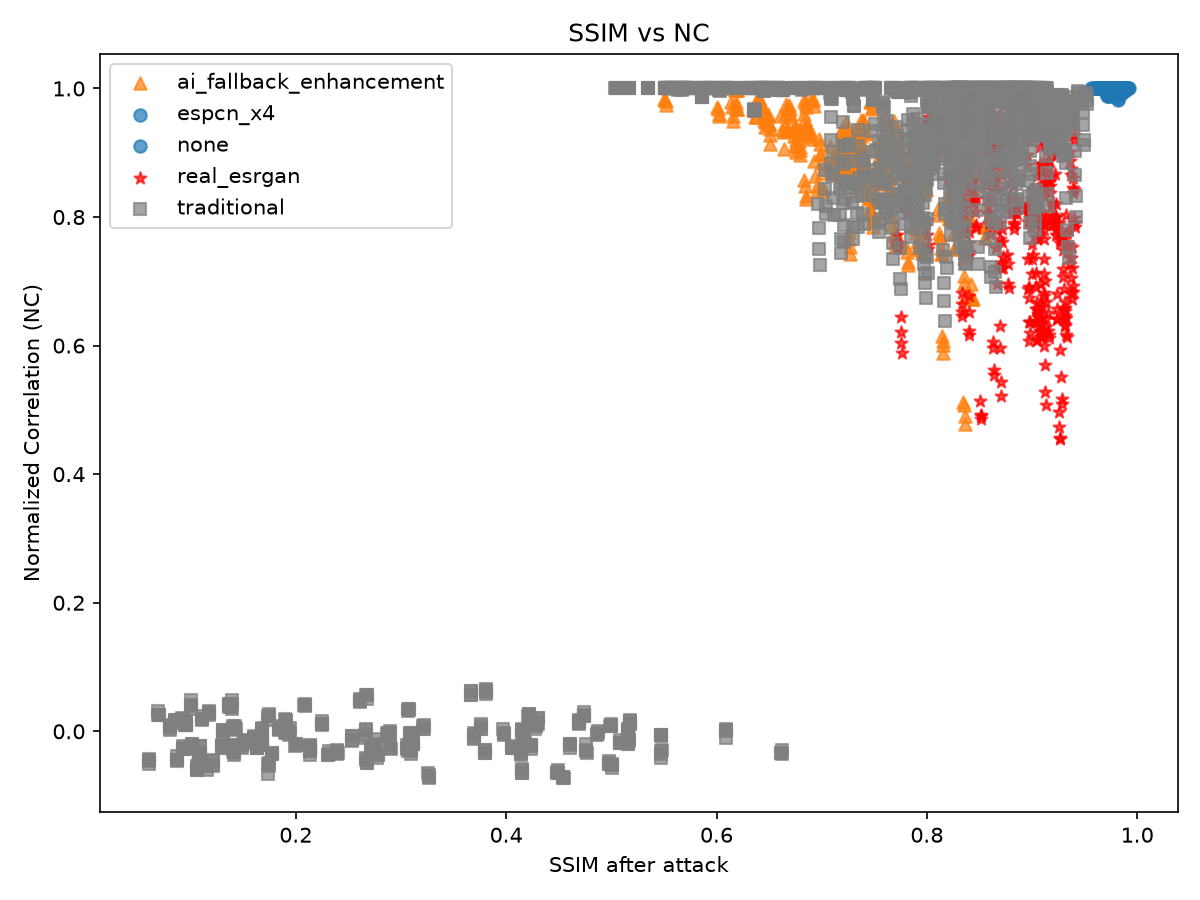
\includegraphics[width=\columnwidth]{figures/ssim_vs_nc.png}
\caption{SSIM vs.\ NC per attacked image. Real-ESRGAN occupies a
high-SSIM, low-NC region unreachable by any classical attack; ESPCN
clusters near $\mathrm{NC}=1.0$ at high SSIM. Classical attacks that
reduce NC also reduce SSIM.}
\label{fig:asymmetry}
\end{figure}

\subsection{The Asymmetry}
Figure~\ref{fig:asymmetry} shows the central observation. Every
classical attack that produces low NC also produces low SSIM ---
watermark damage is coupled to visible quality damage. Real-ESRGAN
decouples them, occupying a high-quality, low-detection region that no
classical attack reaches. Operationally, a content owner monitoring
watermark integrity would observe degraded detection with no visible
indication that the image had been modified. This asymmetry, rather
than the magnitude of NC loss alone, is what distinguishes
enhancement from the classical attack repertoire.

\subsection{Embedding Strength Does Not Restore Robustness}
\begin{table}[t]
\caption{Mean NC under Real-ESRGAN by embedding strength $\alpha$.}
\label{tab:alpha}
\centering
\begin{tabular}{ccc}
\toprule
$\alpha$ & NC (Real-ESRGAN) & SSIM \\
\midrule
0.05 & 0.787 & 0.907 \\
0.10 & 0.797 & 0.906 \\
0.20 & 0.815 & 0.906 \\
0.30 & 0.832 & 0.905 \\
\bottomrule
\end{tabular}
\end{table}
Table~\ref{tab:alpha} shows NC improves only marginally as $\alpha$
quadruples from 0.05 to 0.30, while SSIM remains flat. For classical
attacks, stronger embedding buys proportionally better survival;
Real-ESRGAN does not exhibit this behavior. This is consistent with
the model overwriting the DCT coefficient relationships used for bit
encoding during reconstruction, rather than attenuating the watermark
signal --- an interpretation the next section examines directly.

\section{Mechanism and Mitigation}
\label{sec:analysis}

\subsection{Why: DCT Coefficient Damage Profiles}
\begin{figure}[t]
\centering
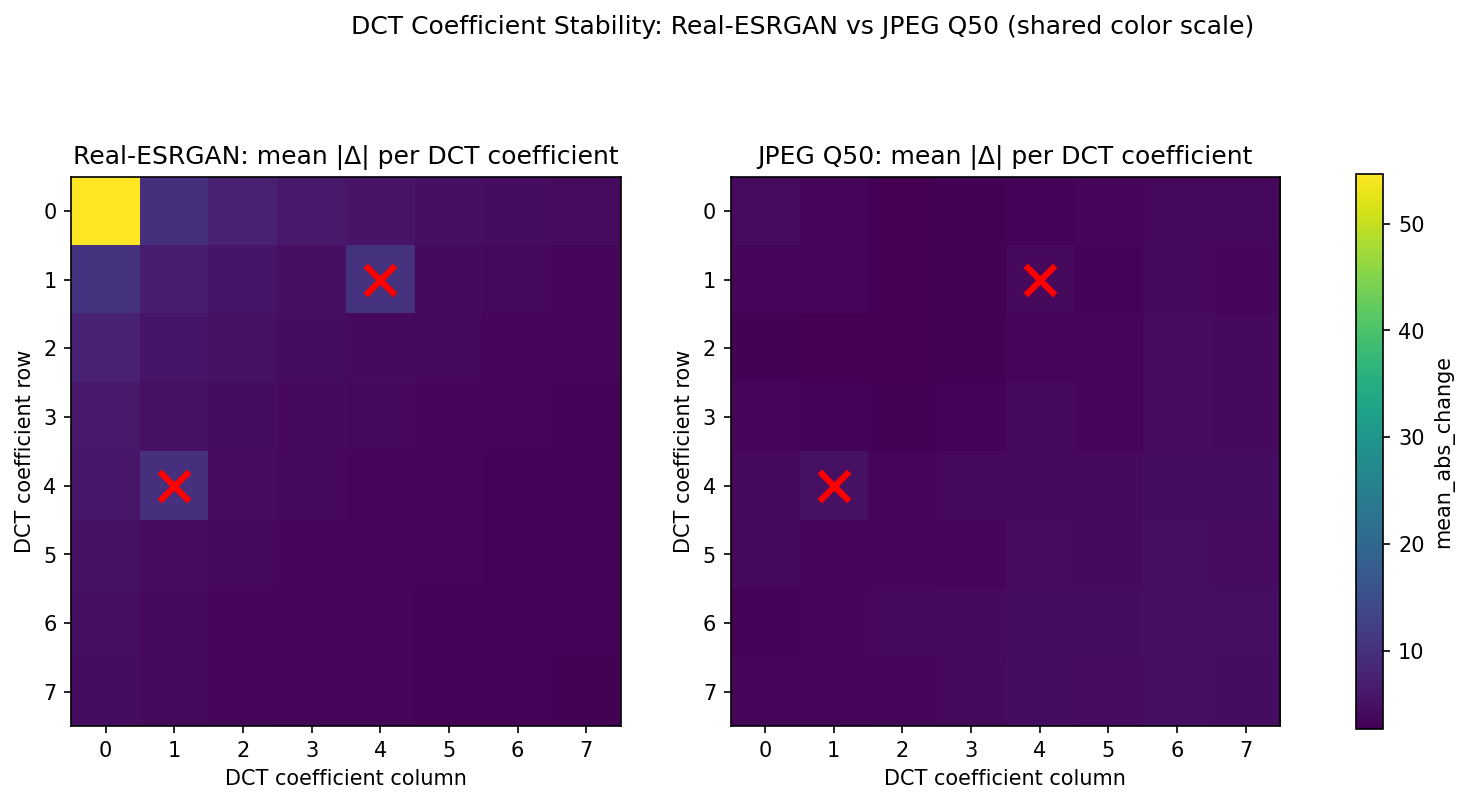
\includegraphics[width=\columnwidth]{figures/dct_stability_comparison.png}
\caption{Mean absolute DCT coefficient perturbation per position for
Real-ESRGAN (left) and JPEG-Q50 (right) across 102,400 blocks, shared
color scale. Real-ESRGAN concentrates damage in the DC coefficient;
JPEG distributes damage nearly uniformly. Baseline embedding positions
$(4,1)$ and $(1,4)$ are marked.}
\label{fig:heatmap}
\end{figure}

Figure~\ref{fig:heatmap} shows mean absolute perturbation per DCT
position. Real-ESRGAN concentrates damage almost entirely in the DC
coefficient at $(0,0)$, with mean perturbation roughly 5 to 14 times
greater than any other position, and elevated perturbation extending
into the low- and mid-frequency region. This pattern is consistent
with the learned reconstruction re-rendering local luminance
statistics; notably, it cannot be attributed to the
upscale--downscale resampling itself, since ESPCN shares that pipeline
and leaves extraction nearly perfect. JPEG-Q50, by contrast,
distributes damage across all 64 positions in a narrow range with
mild elevation at higher frequencies, consistent with its quantization
table design.

The design consequence is direct: the classical embedding positions
$(4,1)$ and $(1,4)$ --- well chosen under JPEG's uniform profile ---
sit in a mid-frequency zone where Real-ESRGAN's perturbation is
elevated relative to the most stable high-frequency corner positions.
The coefficient-selection assumptions inherited from the compression
era do not transfer to the enhancement threat. If damage profiles are
attack-specific, coefficient selection should be attack-aware; the
remainder of this section evaluates that principle.

\subsection{Validation: Frequency Sweep}
\begin{table}[t]
\caption{Mean NC by coefficient-pair symmetry category (20-image
screening set, $\alpha=0.1$).}
\label{tab:symmetry}
\centering
\begin{tabular}{lcccc}
\toprule
Category & ESRGAN & JPEG & Blur & Overall \\
\midrule
Symmetric      & 0.821 & 0.866 & 0.959 & 0.911 \\
Near-symmetric & 0.856 & 0.721 & 0.976 & 0.888 \\
Asymmetric     & 0.689 & 0.868 & 0.735 & 0.822 \\
\bottomrule
\end{tabular}
\end{table}

\textbf{Symmetry.} Symmetric pairs achieve mean NC of 0.821 under
Real-ESRGAN versus 0.689 for asymmetric pairs
(Table~\ref{tab:symmetry}), disconfirming the hypothesis that
coordinate symmetry contributes to the vulnerability.

\textbf{High-frequency corner pairs.} The top-performing pairs under
Real-ESRGAN are anchored at the corner position $(7,7)$, consistent
with the damage profile of Figure~\ref{fig:heatmap}: $(7,5)/(7,7)$
achieves $\mathrm{NC}=0.864$ on the screening set. Re-evaluated across
all 100 images at all four $\alpha$ values, this pair improves
Real-ESRGAN NC from 0.795 to 0.833, at the cost of JPEG regression
from 0.996 to 0.903.

\textbf{Imperceptibility.} The repositioning also carries an
unambiguous benefit: baseline positions $(4,1)/(1,4)$ produce a
minimum per-image PSNR of 36.71\,dB, below the conventional 40\,dB
imperceptibility threshold on some images, whereas $(7,5)/(7,7)$
achieves a minimum of 41.56\,dB, maintaining imperceptibility across
all tested images.

\begin{figure}[t]
\centering
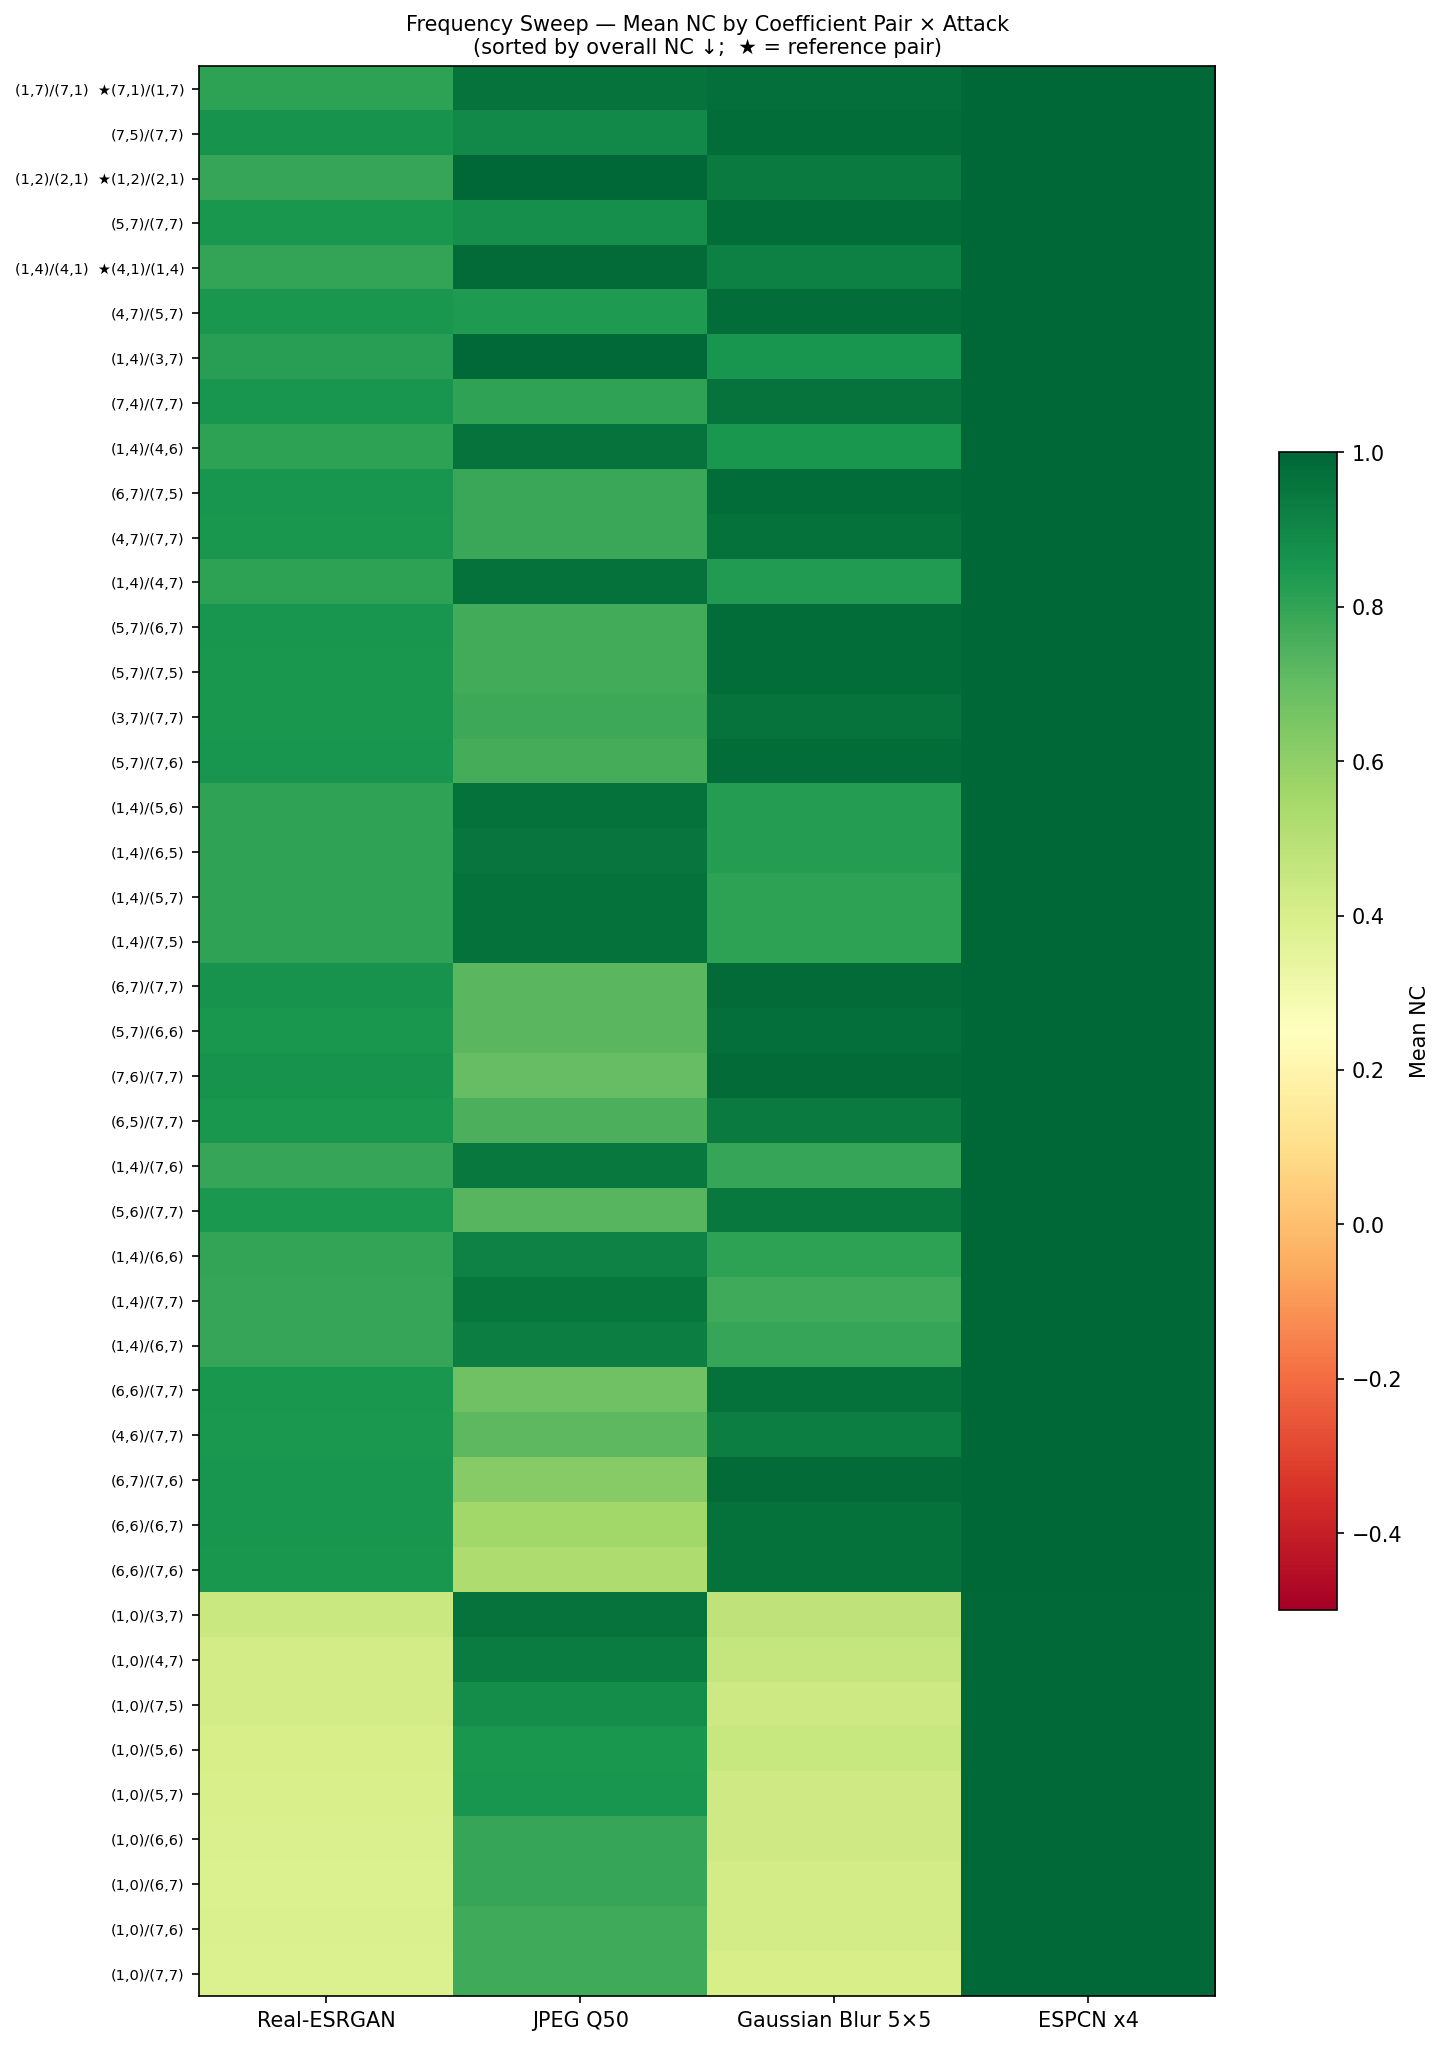
\includegraphics[width=\columnwidth]{figures/frequency_sweep_heatmap.png}
% TODO: confirm filename — this should be the Real-ESRGAN NC vs
% JPEG NC per-pair scatter (Pareto plot), not the position heatmap.
\caption{Real-ESRGAN NC vs.\ JPEG-Q50 NC per coefficient pair. No
pair dominates both axes simultaneously, consistent with a tradeoff
between AI-enhancement and compression robustness.}
\label{fig:pareto}
\end{figure}

\textbf{No universal improvement.} No configuration improves against
all three attacks simultaneously (Figure~\ref{fig:pareto}): pairs that
improve Real-ESRGAN survival regress under compression. Embedding
position selection provides partial, attack-aware mitigation, not a
resolution of the vulnerability.

\subsection{Subband Selection Does Not Help}
As a supplementary comparison, we evaluated a DWT-SVD scheme embedding
in the HH subband at matched imperceptibility (47.7 vs.\ 48.0\,dB
PSNR). It achieves NC of only 0.18 under Gaussian blur and JPEG-Q50
and 0.29 under Real-ESRGAN --- near-chance extraction under attacks
the DWT-DCT-LL scheme survives at 0.93, 0.98, and 0.75 respectively.
Because this comparison changes both the transform (DCT to SVD) and
the subband (LL to HH), it cannot isolate the subband's contribution;
it does, however, suggest that moving embedding energy to
high-frequency subbands is not by itself a viable escape from the
enhancement vulnerability.

\subsection{Limitations}
Our evaluation covers two enhancement architectures; characterizing
enhancement as a general attack category will require evidence across
a broader model family, and our results themselves show the threat is
architecture-specific. All results are reported as means across 100
images without variance estimates. The evaluation targets one
classical scheme (DWT-DCT with ordering-based bit encoding);
generalization to other classical schemes remains to be established.
The frequency sweep screens candidates on a 20-image subset before
full validation of the selected pair, so sweep-level comparisons
(Table~\ref{tab:symmetry}) carry lower statistical weight than the
headline results.

\section{Conclusion}
\label{sec:conclusion}

We investigated whether AI-based image enhancement violates the
quality--attack tradeoff underlying classical watermark robustness
evaluation, and found that it can: Real-ESRGAN degrades DWT-DCT
watermark recovery to $\mathrm{NC}=0.795$ while producing the highest
perceptual quality of any attack tested, a region no classical attack
reaches, while ESPCN --- sharing the identical resampling pipeline ---
leaves watermarks intact. The mechanism is a DC-concentrated
perturbation profile fundamentally unlike JPEG's uniform profile,
under which classically chosen embedding positions are no longer well
placed. Attack-aware repositioning to $(7,5)/(7,7)$ recovers part of
the loss and improves worst-case imperceptibility, but at a quantified
cost to compression robustness; no position improves against all
attacks simultaneously.

Content owners relying on DWT-DCT watermarking should be aware that
consumer enhancement tools can silently degrade watermark integrity.
We recommend that robustness evaluation frameworks adopt AI
enhancement as a standard attack category. Future work should
investigate content-adaptive strategies that jointly optimize
coefficient selection and embedding strength against both classical
and enhancement-class attacks, and should extend the evaluation across
a broader family of enhancement models.

\section*{Acknowledgment}
The author used Claude (Anthropic) as an AI coding assistant for
pipeline implementation. All experimental design, analysis, and
writing are the author's own work.

\bibliographystyle{IEEEtran}
\bibliography{references_revised}

\end{document}
